\documentclass[12pt, oneside, a4paper, brazil]{abntex2}
% \usepackage[utf8]{inputenc}
\usepackage[brazil]{babel}
% \usepackage[T1]{fontenc}
\usepackage{fontspec}
\usepackage{setspace}
\usepackage{graphicx}
\usepackage{scalefnt}
\usepackage{float}
\usepackage[a4paper, left=3cm, right=2.5cm, top=3cm, bottom = 2.5cm]{geometry}
\usepackage{hyperref}
\usepackage{listings}
\usepackage{color}
\usepackage{titlesec}
%\usepackage[alf]{abntex2cite}
% \usepackage{times}
\usepackage[scaled]{helvet}
\usepackage{fancyhdr}
\usepackage{lmodern}
\usepackage{lipsum}


%%% Definição de variáveis. %%%
% ---
% Informações de dados para CAPA e FOLHA DE ROSTO
% ---
\titulo{Análise de desempenho de estruturas de dados para um indexador de arquivos}
\autor{Atílio Antônio Dadalto \\ Tiago da Cruz Santos}
\local{Vitória}
\data{2019}
\instituicao{%
  Universidade Federal do Espírito Santo
  \par Departamento de Informática}
\tipotrabalho{Relatório}
\preambulo{Relatório apresentado como requisito parcial para aprovação na disciplina de Programação I, pela Universidade Federal do Espírito Santo.}

\newcommand{\versao}{2.0}
\newcommand{\subtitulo}{Anteprojeto}


%--- Configurações do environment lstlisting ---
\newfontfamily{\consolas}{Consolas.ttf}

\definecolor{gray}{rgb}{0.5,0.5,0.5}

\lstset{
  language=C,
  basicstyle=\footnotesize\consolas,
  numbers=left,
  numberstyle=\tiny,
  frame=tb,
  tabsize=4,
  breaklines=true,
  postbreak=\mbox{\textcolor{red}{$\hookrightarrow$}\space},
  columns=fixed,
  showstringspaces=false,
  showtabs=false,
  keepspaces,
  commentstyle=\color{gray},
  keywordstyle=\color{blue}
}

% Macros específicas do trabalho.
% (*) Inclua aqui termos que são utilizados muitas vezes e que demandam formatação especial.
% Os exemplos abaixo incluem i* (substituindo o asterisco por uma estrela) e Java com TM em superscript.
% Use sempre \xspace para que o LaTeX inclua espaço em branco após a macro somente quando necessário.
\newcommand{\istar}{\textit{i}$^\star$\xspace}
\newcommand{\java}{Java\texttrademark\xspace}
\newcommand{\latex}{\LaTeX\xspace}


%%% Configurações finais de aparência. %%%

% Altera o aspecto da cor azul.
\definecolor{blue}{RGB}{41,5,195}

% Informações do PDF.
\makeatletter
\hypersetup{
	pdftitle={\@title}, 
	pdfauthor={\@author},
	pdfsubject={\imprimirpreambulo},
	pdfcreator={LaTeX with abnTeX2},
	pdfkeywords={abnt}{latex}{abntex}{abntex2}{trabalho acadêmico}, 
	colorlinks=true,				% Colore os links (ao invés de usar caixas).
	linkcolor=blue,					% Cor dos links.
	citecolor=blue,					% Cor dos links na bibliografia.
	filecolor=magenta,				% Cor dos links de arquivo.
	urlcolor=blue,					% Cor das URLs.
	bookmarksdepth=4
}
\makeatother

% Espaçamentos entre linhas e parágrafos.
\setlength{\parindent}{1.3cm}
\setlength{\parskip}{0.2cm}



%%% Páginas iniciais do documento: capa, folha de rosto, ficha, resumo, tabelas, etc. %%%

% Compila o índice. <--- Desnecessário em Plano de Estudo.
%\makeindex

% Inicia o documento.
\begin{document}

% Retira espaço extra obsoleto entre as frases.
\frenchspacing


% Brasão da instituição.
\begin{figure}[h]
  \centering
  
\includegraphics[scale=0.055]{figuras/brasao}
\end{figure} 

% Capa do trabalho.
\imprimircapa
\imprimirfolhaderosto

% Lista de silgas.
% (*) Indicar as siglas utilizadas no trabalho como no exemplo abaixo.
%\begin{siglas}
    %\item [UML] Linguagem de Modelagem Unificada, do inglês \textit{Unified Modeling Language}
%\end{siglas}

% Índice de capítulos.
\tableofcontents*


%%% Início da parte de conteúdo do documento. %%%

% Marca o início dos elementos textuais.
\clearpage
\textual

% Inclusão dos capítulos.
% (*) Para facilitar a organização, os capítulos foram divididos em arquivo separados e colocados dentro da.
% pasta capitulos/. Caso o aluno prefira trabalhar com um só arquivo, basta substituir os comandos \input 
% pelos conteúdos dos arquivos que estão sendo incluídos, excluindo a pasta capitulos/ em seguida.

\chapter{Introdução}
\label{sec-intro}


Apresenta descrição do problema a ser resolvido e visão geral sobre o funcionamento do programa.
% Exemplos de como usar referência: \citeonline{guarino-et-al:hobook09} (in-line) ou~\cite{guarino-et-al:hobook09}.

\chapter{Implementação}
\label{sec-implementacao}


Descrição sobre a implementação dos algoritmos, incluíndo o algoritmo de Huffman. Deve ser detalhada a estrutura de dados utilizada (de preferência com diagramas ilustrativos), o funcionamento dos algoritmos, e decisões tomadas relativas aos detalhes de especificação que porventura estejam omissos no enunciado.


O pacote \texttt{listings}, incluído neste template, permite a inclusão de listagens de código.  A Listagem NÃO mostra um exemplo de listagem com especificação da linguagem utilizada no código. O pacote \texttt{listings} reconhece algumas linguagens\footnote{Veja a lista de linguagens suportadas em \url{http://en.wikibooks.org/wiki/LaTeX/Source\_Code\_Listings\#Supported_languages}.} e faz ``coloração'' de código (na verdade, usa \textbf{negrito} e não cores) de acordo com a linguagem. O parâmetro \texttt{float=htpb} incluído em ambos os exemplos impede que a listagem seja quebrada em diferentes páginas.

Importante notar que não se deve incluir TODO o código do seu trabalho. Inclua apenas trechos que julgue necessário que sejam discutidos no relatório.


% \lstinputlisting[label=lst-intro-exemplo, caption=Exemplo de código C especificando linguagem utilizada., language=C, float=htpb]{codigos/lst-exemplo.c}

\chapter{Metodologia}\label{cap-metodologia}

% Descrever a metodologia dos testes, como variou o tamanho dos arquivos, quantos arquivos foram utilizados, descrição do computador em que foram feitos os testes.

Utilizando scripts de bash, pudemos automatizar os processos de testes, facilitando muito o levantamento de dados, possibilitando a obtenção de um maior espaço amostral e reduzindo os erros humanos. 

% 20?
Os testes foram realizados executando 20 iterações de um mesmo programa. Por exemplo, um carregamento de 10 arquivos com 500 buscas aleatórias seria repetido 20 vezes. Assim, garantimos que o espaço amostral seja satisfatório para a obtenção de dados pouco enviesados por \textit{outliers} --- neste caso, buscas e inserções muito lentas ou muito rápidas --- sobre a execução do programa.

Além disso, todos os testes foram efetuados em duas máquinas diferentes. A Máquina 1 possui 8GB de RAM e um processador AMD FX-6300 com 6 núcleos rodando a 3.80GHz com um sistema operacional Linux Mint 19.1; já a Máquina 2 conta com 16GB de RAM e um processador Intel i7-7XXX com 8 núcleos rodando a XGHz e um sistema operacional Linux Ubuntu X.

Os arquivos utilizados para testes variaram de 1KB a cerca de 10MB, de 1 a 15 arquivos por vez. Arquivos com mais de 20MB usualmente demoram mais de uma hora para carregar em todas as estruturas, portanto este foi o limite estipulado pelos nossos testes.

\section{Resultados}

Analisar os tamanhos dos arquivos compactados a partir dos experimentos realizados. Utilizar tabelas e gráficos para ilustrar o desempenho da sua implementação.








\begin{comment}

Exemplo de utilização de tabelas.  A Tabela ~\ref{tab:cronograma-1} apresenta um cronograma de execução de um PG fictício.

\begin{table}[htb]
	\centering
	\caption{Cronograma de Atividades do primeiro semestre.}
	\label{tab:cronograma-1}
	\resizebox{\columnwidth}{!}{
		\begin{tabular}{c|c|c|c|c|c|c}
			Atividade & Janeiro/99 & Fevereiro/99  & Março/99  & Abril/99 & Maio/99 & Junho/99\\ \hline
			1&     X      &  	  X   	       &  	X	  	   & 		X	&     X   &      X    \\ \hline
			2&            &  	   	     	   &  	  X  	   & 		X	&         &           \\ \hline
			3&            &  		           &  	  X 	   & 		X   &   X     &     X      \\ \hline
			4&            &  			       &  			   & 	        &         &     X      \\ \hline
			5&            &  			       &  			   & 	        &    X    &   X       \\ \hline
			6&            &  			       &  			   & 	        &         &           \\ \hline
			7&            &  			       &  			   & 	        &         &           \\ \hline
		\end{tabular}
	}
\end{table}

A Figura \ref{fig:graf} exemplifica o uso de uma figura gráfica no texto.

\begin{figure}[!htb]
\centering
%   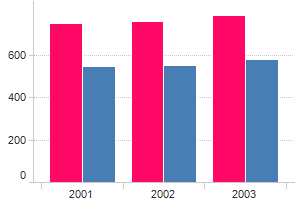
\includegraphics[scale=0.90]{figuras/graf-exemplo.png}
  \caption{Exemplo de inserção de figura}
  \label{fig:graf}
\end{figure}
\end{comment}

\chapter{Metodologia}

Descrever a metodologia dos testes, como variou o tamanho dos arquivos, quantos arquivos foram utilizados, descrição do computador em que foram feitos os testes.

\section{Resultados}

Analisar os tamanhos dos arquivos compactados a partir dos experimentos realizados. Utilizar tabelas e gráficos para ilustrar o desempenho da sua implementação.

Exemplo de utilização de tabelas.  A Tabela ~\ref{tab:cronograma-1} apresenta um cronograma de execução de um PG fictício.


\begin{table}[htb]
	\centering
	\caption{Cronograma de Atividades do primeiro semestre.}
	\label{tab:cronograma-1}
	\resizebox{\columnwidth}{!}{
		\begin{tabular}{c|c|c|c|c|c|c}
			Atividade & Janeiro/99 & Fevereiro/99  & Março/99  & Abril/99 & Maio/99 & Junho/99\\ \hline
			1&     X      &  	  X   	       &  	X	  	   & 		X	&     X   &      X    \\ \hline
			2&            &  	   	     	   &  	  X  	   & 		X	&         &           \\ \hline
			3&            &  		           &  	  X 	   & 		X   &   X     &     X      \\ \hline
			4&            &  			       &  			   & 	        &         &     X      \\ \hline
			5&            &  			       &  			   & 	        &    X    &   X       \\ \hline
			6&            &  			       &  			   & 	        &         &           \\ \hline
			7&            &  			       &  			   & 	        &         &           \\ \hline
		\end{tabular}
	}
\end{table}


A Figura \ref{fig:graf} exemplifica o uso de uma figura gráfica no texto.


   \begin{figure}[!htb]
    \centering
   	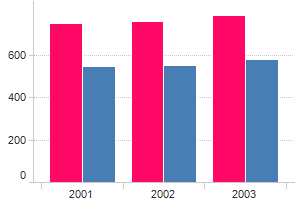
\includegraphics[scale=0.90]{figuras/graf-exemplo.png}
   	\caption{Exemplo de inserção de figura}
   	\label{fig:graf}
   \end{figure}

\chapter*{CONCLUSÃO}\label{cap-conclusao}
\addcontentsline{toc}{chapter}{CONCLUSÃO}

Com os dados levantados e a análise feita, podemos então discutir os resultados de uma forma geral. Apesar de uma amostra de 20 iterações não ser ideal, é o suficiente para tomarmos conclusões sobre os desempenhos.

% por conta de sua inserção que percorre a lista toda em busca de um elemento que seja igual ao elemento a ser inserido 
% Mesmo que as inserções das árvores possuam complexidade computacional grande, estas possuem uma buscas mais velozes que a da lista, por exemplo.
Sendo assim, a lista encadeada, como mostrado no Capítulo~\ref{cap-analise-resultado}, é a estrutura mais lenta dentre todas do projeto, possuindo custo $O(n)$ em vez do $O(1)$ usual para inserções de listas encadeadas. Apesar de tudo, a implementação da lista também é extremamente mais simples comparada às implementações das árvores, o que não ajuda apenas a construção inicial de um projeto, mas também sua manutenção.

A árvore binária sem balanceamento... comparar com outras estruturas

A árvore binária balanceada, por sua vez, demonstrou o desempenho mais equilibrado dentre as cinco estruturas; sua inserção é levemente mais lenta que a da lista encadeada, porém a busca consegue ser extremamente mais rápida, com complexidade $O(\log{n})$ no pior caso. Por conta de seu equilíbrio, foi escolhida para acomodar Palavras na tabela hash.

A árvore de prefixos, ou trie, teve o melhor desempenho de todos para buscas... sera mesmo?¿

Por fim, a tabela hash...

Portanto, cabe ao idealizador de um projeto determinar qual estrutura é mais adequada ao problema em questão, analisando, se possível, a razão entre inserção e busca e também se a solução não é complexa demais para o objetivo proposto. Para um projeto diminuto, a lista encadeada poderia ser utilizada sem problemas notáveis de performance, ainda sendo válido destacar sua simples implementação; no caso de um indexador, no entanto, ela representou a pior estrutura. Como visto na seção... a melhor estrutura para inserções, neste caso, foi a .... Já a melhor para buscas foi a ... (trie?). A estrutura X se demonstrou equilibrada quando inserções e buscas são levadas em consideração em conjunto. Para um projeto como este de um indexador de palavras, os autores consideram a estrutura x como a mais capacitada para o empreendimento.

\lipsum[10]


% Finaliza a parte no bookmark do PDF para que se inicie o bookmark na raiz e adiciona espaço de parte no sumário.
\phantompart

% Marca o fim dos elementos textuais.
\postextual

% Referências bibliográficas
\clearpage
\bibliography{bibliografia}

% Fim do documento.
\end{document}
